%%%%%%%%%%%%%%%%%%%%%%%%%%%%%%%%%%%%%%%%%%%%%%%%%%%%%%%%%%%%%%%%%%%%%%%%%%
%
% StAssociationMaker - User Guide and Reference Manual -- LaTeX Source
%
% $Id: StAssociationMaker.tex,v 1.2 1999/07/14 14:46:13 calderon Exp $
%
% Authors:Michael A. Lisa
%         Thomas S. Ullrich
%         Manuel Calderon de la Barca Sanchez
%
%%%%%%%%%%%%%%%%%%%%%%%%%%%%%%%%%%%%%%%%%%%%%%%%%%%%%%%%%%%%%%%%%%%%%%%%%%
%
% Notes to the authors:
%
% - A template for a class reference is at the end of this file.
% - Wrap all names functions with \name{}
% - All code, examples, prototypes in \verb+ ... +\\
%   or \begin{verbatim} ... \end{verbatim}
% - Use \StAssociationMaker if you refer to the package itself (not the class)
%
% This file is best edit with xemacs and the 'Function' package loaded.
%
%%%%%%%%%%%%%%%%%%%%%%%%%%%%%%%%%%%%%%%%%%%%%%%%%%%%%%%%%%%%%%%%%%%%%%%%%%
%
% $Log: StAssociationMaker.tex,v $
% Revision 1.2  1999/07/14 14:46:13  calderon
% Updated documentation to include macros in CVS
%
%
%%%%%%%%%%%%%%%%%%%%%%%%%%%%%%%%%%%%%%%%%%%%%%%%%%%%%%%%%%%%%%%%%%%%%%%%%%
\documentclass[twoside]{article}

\parindent 0pt
\parskip 6pt
\advance\textwidth by 80pt%
\advance\evensidemargin by -80pt%

\usepackage{graphicx}
\usepackage{psboxit}
\usepackage{amsmath}
\usepackage{amssymb}
\usepackage{amsfonts}
\usepackage{fancyhdr}
\usepackage{times}
\usepackage{verbatim}
\usepackage{makeidx}

\PScommands      % init boxit
\makeindex

%%%%%%%%%%%%%%%%%%%%%%%%%%%%%%%%%%%%%%%%%%%%%%%%%%%%%%%%%%%%%%%%%%%%
%
% Define header and footer style
%
%%%%%%%%%%%%%%%%%%%%%%%%%%%%%%%%%%%%%%%%%%%%%%%%%%%%%%%%%%%%%%%%%%%%
\pagestyle{fancyplain}
\rhead[\fancyplain{}{\bfseries\leftmark}]
      {\fancyplain{}{\bfseries\rightmark}}
\lhead[\fancyplain{}{\bfseries\rightmark}]
      {\fancyplain{}{\bfseries\leftmark}}
\rfoot[{}]{\fancyplain{}{\bfseries\thepage}}
\lfoot[\fancyplain{}{\bfseries\thepage}]{}
\cfoot{}

%%%%%%%%%%%%%%%%%%%%%%%%%%%%%%%%%%%%%%%%%%%%%%%%%%%%%%%%%%%%%%%%%%%%
%
% Typographic Conventions
%
%%%%%%%%%%%%%%%%%%%%%%%%%%%%%%%%%%%%%%%%%%%%%%%%%%%%%%%%%%%%%%%%%%%%
\newcommand{\name}[1]{\textsl{#1}}%  class-, function-, package names
\newcommand{\StEvent}{\textsf{StEvent}}
\newcommand{\StMcEvent}{\textsf{StMcEvent}}
\newcommand{\StAssociationMaker}{\textsf{StAssociationMaker}}
\newcommand{\StMcAnalysisMaker}{\textsf{StMcAnalysisMaker}}

%%%%%%%%%%%%%%%%%%%%%%%%%%%%%%%%%%%%%%%%%%%%%%%%%%%%%%%%%%%%%%%%%%%%
%
% Define multiline labels for class reference
%
%%%%%%%%%%%%%%%%%%%%%%%%%%%%%%%%%%%%%%%%%%%%%%%%%%%%%%%%%%%%%%%%%%%%
\newcommand{\entrylabel}[1]{\mbox{\textbf{{#1}}}\hfil}%
\newenvironment{entry}
{\begin{list}{}%
    {\renewcommand{\makelabel}{\entrylabel}%
     \setlength{\labelwidth}{90pt}%
     \setlength{\leftmargin}{\labelwidth}
     \advance\leftmargin by \labelsep%
    }%
}%
{\end{list}}

\newcommand{\Entrylabel}[1]%
{\raisebox{0pt}[1ex][0pt]{\makebox[\labelwidth][l]%
    {\parbox[t]{\labelwidth}{\hspace{0pt}\textbf{{#1}}}}}}
\newenvironment{Entry}%
{\renewcommand{\entrylabel}{\Entrylabel}\begin{entry}}%
  {\end{entry}}

\begin{document}

%%%%%%%%%%%%%%%%%%%%%%%%%%%%%%%%%%%%%%%%%%%%%%%%%%%%%%%%%%%%%%%%%%%%
%
%    Title page
%
%%%%%%%%%%%%%%%%%%%%%%%%%%%%%%%%%%%%%%%%%%%%%%%%%%%%%%%%%%%%%%%%%%%%
\begin{titlepage}
\pagestyle{empty}
\vspace*{-35mm}
\begin{center}
  \mbox{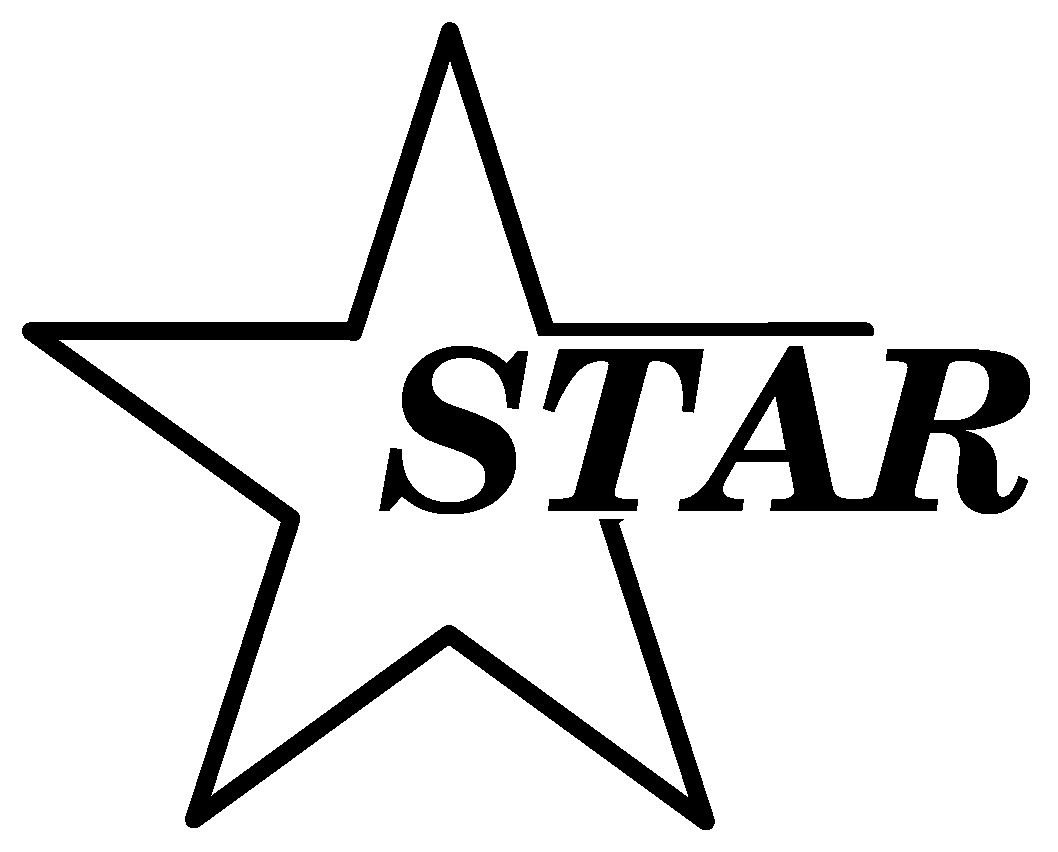
\includegraphics[width=2cm]{StarIcon.eps}}
  {\Large\bf STAR Offline Library Long Writeup}
  \hfill\mbox{}\\[3cm]
  \mbox{\includegraphics[width=\textwidth]{StAssociationMakerTitle.eps}}
  \hfill\mbox{}\\[3cm]
  {\LARGE User Guide and Reference Manual}\\[2cm]
  {\LARGE $  $}  \\[5mm] % replaced by cvs with current revision
  {\LARGE $  $}  % replaced by cvs with current revision
  \vfill
\end{center}
\cleardoublepage
\end{titlepage}
\pagenumbering{roman}

%%%%%%%%%%%%%%%%%%%%%%%%%%%%%%%%%%%%%%%%%%%%%%%%%%%%%%%%%%%%%%%%%%%%
%
%    Table of contents
%
%%%%%%%%%%%%%%%%%%%%%%%%%%%%%%%%%%%%%%%%%%%%%%%%%%%%%%%%%%%%%%%%%%%%
\tableofcontents
\cleardoublepage

%%%%%%%%%%%%%%%%%%%%%%%%%%%%%%%%%%%%%%%%%%%%%%%%%%%%%%%%%%%%%%%%%%%%
%
%    User Guide
%
%%%%%%%%%%%%%%%%%%%%%%%%%%%%%%%%%%%%%%%%%%%%%%%%%%%%%%%%%%%%%%%%%%%%
\pagenumbering{arabic}
\part{User Guide}
\clearpage

%%%%%%%%%%%%%%%%%%%%%%%%%%%%%%%%%%%%%%%%%%%%%%%%%%%%%%%%%%%%%%%%%%%%

\section{Introduction}

\StAssociationMaker\footnote{We will adopt the convention used in \StEvent\ 
    and write \StMcEvent\ when we refer to the package and
    \name{StMcEvent} when we refer to the class.} is a package that
uses the functionality of \StEvent\ and \StMcEvent\ together in order
to have reconstructed and Monte Carlo information handy.
The package is called after both \StEvent\ and \StMcEvent\ have been loaded
in a ROOT session for a given event.  
\index{StAssociationMaker}
The aim of \StAssociationMaker\ is to establish the relationships, based
on certain criteria, between the reconstructed and Monte Carlo information.
In this way,
users can easily check whether a particular reconstructed hit or
track came from a Monte Carlo object, and directly obtain the associated Monte
Carlo hit or track so that an assessment of the quality of the
data can be made.

\clearpage

%%%%%%%%%%%%%%%%%%%%%%%%%%%%%%%%%%%%%%%%%%%%%%%%%%%%%%%%%%%%%%%%%%%%

\section{How to read this document}

This document is divided in two parts, a user guide and a
reference manual. The first part is the main part, since although
the package contains several classes, the only class that is designed
for general use is \name{StAssociationMaker}.  Apart from the usual
methods provided for makers, this class has only a few additional methods
for general use: the methods to access the multimaps.  The navigation and
use of \StEvent\ and \StMcEvent\ are described in their respective
documentation.
This manual will cover these methods, and how to
use the package.  The user guide will also provide an explanation of
the \StMcAnalysisMaker\ package.  This additional package is basically
a working example.  The class reference will be kept short for the
reasons described above.

Understanding the various
examples certainly is the best way to get started. In this case,
\StMcAnalysisMaker\ is actually a working example.  It can be
run with the macro \name{StAssociator.C} .
%%%%%%%%%%%%%%%%%%%%%%%%%%%%%%%%%%%%%%%%%%%%%%%%%%%%%%%%%%%%%%%%%%%%

\section{Further documentation}
\label{sec:furtherdoc}

\StAssociationMaker\ makes use of various classes from the StarClassLibrary (SCL).
To obtain the SCL documentation perform the following steps:
\begin{enumerate}
  \item Obtain an \name{afs} token: \name{klog -cell rhic}.
  \item Make sure \name{\$CVSROOT} is set properly: \\ %%$
	(i.e.~\name{CVSROOT = /afs/rhic/star/packages/repository})
  \item Check-out the SCL into your current working directory:\\
    \name{cvs checkout StRoot/StarClassLibrary}
  \item Go to the directory containing the documentation:\\
    \name{cd StRoot/StarClassLibrary/doc/tex}
  \item Create the PostScript document \name{StarClassLibrary.ps}:\\
    \name{make}
\end{enumerate}
\index{SCL} \index{StarClassLibrary}

%%%%%%%%%%%%%%%%%%%%%%%%%%%%%%%%%%%%%%%%%%%%%%%%%%%%%%%%%%%%%%%%%%%%

\section{Getting \StAssociationMaker\ Sources}  \index{Getting StAssociationMaker sources}

To access the complete source code proceed as follows:

\StAssociationMaker\ is under {\bf CVS} control at BNL.  It can
be accessed via \name{afs}: \index{afs} \index{CVS} \index{CVSROOT}
\begin{enumerate}
  \item Obtain an \name{afs} token: \name{klog -cell rhic}.
  \item Make sure \name{\$CVSROOT} is set properly:\\ %%$
    (i.e.~\name{CVSROOT = /afs/rhic/star/packages/repository})
  \item Check-out package into your current working directory:\\
    \name{cvs checkout StRoot/StAssociationMaker}
  \item Check-out the examples
    \name{cvs checkout StRoot/StMcAnalysisMaker}
  \item Copy the macro your current working directory:
    \name{cp \$STAR/StRoot/macros/StAssociator.C /.} %$
\end{enumerate}

%%%%%%%%%%%%%%%%%%%%%%%%%%%%%%%%%%%%%%%%%%%%%%%%%%%%%%%%%%%%%%%%%%%%

\section{How it works: a quick overview of multimaps}
\label{sec:howitworks}
\index{multimap}
A multimap \footnote{For reference look in Stroustrup's C++ book, 3d Ed. pp. 484-490}  is a type of associative container that allows for duplicate keys.
That is, it can be thought of as a collection of pairs of objects that are queried based on the first
element of the pair (the KEY). \index{KEY for a multimap}  This implies that simple
subscripting by key values (like an array) is not supported.  The main way to access
the multiple values given to a single key is then through iterators.  These iterators
are obtained through the operations \name{upper\_bound()}, \name{lower\_bound()}, and
\name{equal\_range()}.
For a multimap \name{lower\_bound(k)} and \name{upper\_bound(k)} give the beginning
and end of the subsequence of elements of the map that have the key ``k''.  However,
as Stroustrup says, doing 2 operations all the time is neither elegant nor efficient.  The
operation \name{equal\_range(k)} is provided to deliver both.  For examples of this usage 
refer to sec.~\ref{sec:howto}. 

The multimaps used in \StAssociationMaker\ 
keep a relationship between the reconstructed \StEvent\ objects and Monte Carlo
\StMcEvent\ objects.  This
relationship is established starting from the hit information and building up
from there.

The criterion for associating a given reconstructed hit to a \index{Hit association}
Monte Carlo hit is based on their spatial proximity.  We use x and z coordinates
of the hits and make a cut.  The default value of the cuts are 1 millimeter for
each direction.  However, users can set their own criteria at the macro level.  This
is done so that when one wants to change this value, it is not necessary to recompile
the package.

Once the hit associations are made, the criterion for associating a
reconstructed track to a Monte Carlo track is \index{Track association}
based on the number of hits they have in common.  The default value is 3.  We wanted
to keep this number loose so the map would really rule out bad associations but keep
enough tracks in the map to make further analysis using the map.  Therefore the structure
of the track map is a little different than the hit map.  Instead of just associating an
\name{StGlobalTrack} to an \name{StMcTrack}, we make the association between an
\name{StGlobalTrack} and an instance of an \name{StTrackPairInfo} class. \index{StTrackPairInfo}
This class has,
of course, a pointer to the associated \name{StMcTrack} but in additon has a member that
keeps track of the number of hits the 2 tracks have in common.  This is done so that
later on one can make more stringent cuts on the tracks.  If any additional information
is needed, we would only modify the \name{StTrackPairInfo} class to accomodate it.  Moreover,
the default value of 3 required hits in common can also be modified at the macro level.

The cuts are kept in an instance of the singleton class \name{StMcParameterDB}.  This
class is instantiated exactly once (hence the name ``singleton'') and the rest of
the classes in \StAssociationMaker\ look there to figure out the cut criteria.
For an example of how to change the cuts, look in the \name{StAssociator.C}
macro.  


%%%%%%%%%%%%%%%%%%%%%%%%%%%%%%%%%%%%%%%%%%%%%%%%%%%%%%%%%%%%%%%%%%%%


\section{How to use it: StMcAnalysisMaker and StAssociator.C}
\label{sec:howto}
\index{StAssociator.C}
\index{StMcAnalysisMaker}
\index{root4star}
\index{ROOT files}
The procedure starting from scratch to run the provided 
example is (Note that \StAssociationMaker\ runs at the moment
only on Linux and in new):
\begin{verbatim}
    ssh coburn 
    starnew
    mkdir workdir
    cd workdir
    cvs co StRoot/StMcEvent
    cvs co StRoot/StMcEventMaker
    cvs co StRoot/StAssociationMaker
    cvs co StRoot/StMcAnalysisMaker
    makel -C StRoot/StMcEvent
    makel -C StRoot/StMcEventMaker
    makel -C StRoot/StAssociationMaker
    makel -C StRoot/StMcAnalysisMaker
    root4star StAssociator.C
\end{verbatim}

Please note that at the moment, StMcEventMaker only runs with ROOT files.

StAssociator.C can be found in \name{\$CVSROOT/StRoot/macros/examples/StAssociator.C}, %$%%%
and it runs a 
chain consisting of four makers:
\begin{description}
\item[\name{StEventReaderMaker}:] loads StEvent
\item[\name{StMcEventMaker}:] loads StMcEvent
\item[\name{StAssociationMaker}:] creates the hit and track associations
\item[\name{StMcAnalysisMaker}:] Picks up the previous info. and analyzes it 
    (incorporates a few simple examples)
\end{description}

%%%%%%%%%%%%%%%%%%%

At the moment, it runs the chain on a ROOT file tree.  That is, it uses the DST
and GEANT braches of the files it finds in the directory.  Example invocation
is 
\begin{verbatim}
.x StAssociator.C(10,"-",
    "/disk00000/star/test/new/tfs_Solaris/year_2a/psc0210_01_40evts.geant.root")

   processes 10 events from the specified file

\end{verbatim}
It takes the path to look for files from the specified file, but the files it
actually opens depend on
what branches are activated in the macro.
This is done inside the macro with the command \name{SetBranch}.


\subsection{StMcAnalysisMaker::Make()}
We will explain here the first example in
the \name{Make()} method of \name{StMcAnalysisMaker}, since this is the
part that most users will follow.
Recall that when \name{StMcAnalysisMaker::Make()} is called, the following should have already
happened:
\begin{enumerate}
\item \StEvent\ should be loaded in the chain.
\item \StMcEvent\ should be loaded in the chain.
\item \StAssociationMaker\ should have finished making associations.
\end{enumerate}

We need to access the packages and information that is already loaded.  This is done
by getting a pointer to \name{StEvent}, a pointer to \name{StMcEvent}, and a pointer
to \name{StAssociationMaker}:

\begin{verbatim}
    // Get the pointers we need, we have to use the titles we gave them in the
    // macro.  I just used the defaults.
    StEvent* rEvent = 0;
    rEvent = ((StEventMaker*) gStChain->Maker("events"))->event();
    StMcEvent* mEvent = 0;
    mEvent = ((StMcEventMaker*) gStChain->Maker("MCEvent"))->currentMcEvent();
    StAssociationMaker* assoc = 0;
    assoc = (StAssociationMaker*) gStChain->Maker("Associations");
\end{verbatim}

The pointer to \name{StAssociationMaker} then enables us to get the pointers to the
appropriate multimpas:

\begin{verbatim}

    tpcHitMapType* theHitMap = 0;
    theHitMap = assoc->tpcHitMap();
    trackMapType* theTrackMap = 0;
    theTrackMap = assoc->trackMap();

\end{verbatim}

The classes \name{tpcHitMapType} and \name{trackMapType} are the typedef's to the
appropriate multimaps.  \index{tpcHitMapType} \index{trackMapType} 
We see here that to get a the pointers to them we just need to call
the \name{StAssociationMaker::tpcHitMap()} and \name{StAssociationMaker::trackMap()} methods.

Once we have the pointers to the maps, we can start analyzing them.  The first example
in the maker shows how to check whether a particular reconstructed TPC Hit was associated
with a Monte Carlo hit. 

\begin{verbatim}

 // Example: look at hits associated with 1st REC hit in Tpc Hit collection.

 StTpcHit*     firstHit;
 firstHit = *( rEvent->tpcHitCollection()->begin() );
 cout << "Assigned First Hit: " << endl;
 cout << *firstHit << endl;
 cout << "This hit has " <<  theHitMap->count(firstHit);
 cout << " MC Hits associated with it."<< endl;

 // To get the associated hits of the first hit we use equal_range(key),
 // which returns 2 iterators, the lower bound and upper bound,
 // so that then we can loop over them.
    
 cout << "Position of First Rec. Hit and Associated (if any) MC Hit:" << endl;
 pair<tpcHitMapIter,tpcHitMapIter> hitBounds = theHitMap->equal_range(firstHit);

 for (tpcHitMapIter it=hitBounds.first; it!=hitBounds.second; ++it) {
    cout << "[" << (*it).first->position();
    cout << ", "<< (*it).second->position() << "]" << endl;
 }
\end{verbatim}

The other examples in the maker show
\begin{enumerate}
\item how to make a histogram using the Hit multimap
\item how to use an \name{StGlobalTrack} to get its partner in the Track multimap.
\item how to make a histogram using the Track multimap
\end{enumerate}

(Note that the histograms were defined in the header file as public data members.)

To play with it yourself you can pick up StMcAnalysisMaker and 
use it as a template for a Maker of your own that works with
StMcEvent:

\begin{verbatim}
    mkdir StRoot/StMyMcAnalysisMaker
    cp  $STAR/StRoot/StMcAnalysisMaker/* StRoot/StMyMcAnalysisMaker/                                   %$
    [edit]
    makel -C StRoot/StMyMcAnalysisMaker
    cvs co $CVSROOT/StRoot/macros/examples/StAssociator.C  (and edit to use your maker)                            %$
    root4star StAssociator.C
\end{verbatim}

%%%%%%%%%%%%%%%%%%%%%%%%%%%%%%%%%%%%%%%%%%%%%%%%%%%%%%%%%%%%%%%%%%%%


\section{Known Problems} \index{known problems (\StAssociationMaker\ )}

\StAssociationMaker\ is not yet complete.  
It has only been tested in new, SL99e.  We do not foresee
to make it work in dev (SL99f) since \StEvent\ itself is going through a major
overhaul.  The next version will be developed once the new \StEvent\
is in place, and also the changes in the g2t\_vertex table have been
implemented.

The FTPC and SVT associations between reconstructed and Monte Carlo
hits are not included presently (although the appropriate Collections are
filled by \name{StMcEventMaker} ). 
Also, \StAssociationMaker\ does not compile with SUN CC4.2 yet, because
that compiler has problems handling multimaps, and this is being worked on.


\clearpage

%%%%%%%%%%%%%%%%%%%%%%%%%%%%%%%%%%%%%%%%%%%%%%%%%%%%%%%%%%%%%%%%%%%%
%
%    Reference Manual
%
%%%%%%%%%%%%%%%%%%%%%%%%%%%%%%%%%%%%%%%%%%%%%%%%%%%%%%%%%%%%%%%%%%%%
\part{Reference Manual}
\label{refman}
\clearpage

%%%%%%%%%%%%%%%%%%%%%%%%%%%%%%%%%%%%%%%%%%%%%%%%%%%%%%%%%%%%%%%%%%%%

\section{Global Constants}

We use the constants defined in the two header files
\index{StarClassLibrary} \name{SystemOfUnits.h} and
\name{PhysicalConstants.h} which are part of the StarClassLibrary.
The types defined therein are used
throughout \StMcEvent\ .

%%%%%%%%%%%%%%%%%%%%%%%%%%%%%%%%%%%%%%%%%%%%%%%%%%%%%%%%%%%%%%%%%%%%


\section{Class Reference}
The classes which are currently implemented and available from the
STAR CVS repository are described in alphabetic order.  Only the
classes normally accessible to users are described.

\clearpage


%%%%%%%%%%%%%%%%%%%%%%%%%%%%%%%%%%%%%%%%%%%%%%%%%%%%%%%%%%%%%%%%%%%%
%
%    Reference: StAssociationMaker
%
%%%%%%%%%%%%%%%%%%%%%%%%%%%%%%%%%%%%%%%%%%%%%%%%%%%%%%%%%%%%%%%%%%%%
\subsection{StAssociationMaker}
\index{StAssociationMaker|textbf}
\index{event header}
\label{sec:StAssociationMaker}
\begin{Entry}
\item[Summary]
    \name{StAssociationMaker} is the main class in the \StAssociationMaker\ package.
    It aim is to create the multimaps, and to provide methods to access them. 

\item[Synopsis]
    \verb+#include "StAssociationMaker.h"+\\
    \verb+class StAssociationMaker;+\\

\item[Description]
    Objects of type \name{StAssociationMaker} are the entry point to the hit
    and track multimaps.
    From here one can navigate to (and access) quantities stored
    in them.  Of course, one normally needs to include the necessary
    \StEvent\ and \StMcEvent\ classes to use in one's own analysis maker.

\item[Persistence]
    None

\item[Related Classes]
    None

\item[Public\\ Constructors]
    \verb+StAssociationMaker(const char* name = "Associations",const char* title = "event/Associations");+\\
		       
    Maker constructor.

\item[Public Member\\ Functions]
    

    \verb+virtual void Clear(const char* opt="");+\\
    Deletes the multimaps and the single histogram data member.  Then calls standard Clear() for makers. 
    \index{Clear()}

    \verb+virtual Int_t Init();+\\
    Standard for makers. 
    \index{Init()}

    \verb+virtual Int_t Make();+\\
    Makes hit and track associations, i.e. builds the multimaps.
    \index{Make()}

    \verb+virtual Int_t Finish();+\\
    Standard for makers.
    \index{Finish()}

    \verb+tpcHitMapType* tpcHitMap();+\\
    Returns the pointer to the TPC Hit multimap.  This is the way to get access to
    the map from another maker.  Look in sec.~\ref{sec:howto}
    \index{tpcHitMap()}

    \verb+trackMapType* trackMap()+\\
    Returns the pointer to the Track multimap.  This is the way to get access to
    the map from another maker.  Look in sec.~\ref{sec:howto}
    \index{trackMap()}

\end{Entry}

%%%%%%%%%%%%%%%%%%%%%%%%%%%%%%%%%%%%%%%%%%%%%%%%%%%%%%%%%%%%%%%%%%%%
%
%    Reference: StMcParameterDB
%
%%%%%%%%%%%%%%%%%%%%%%%%%%%%%%%%%%%%%%%%%%%%%%%%%%%%%%%%%%%%%%%%%%%%
\subsection{StMcParameterDB}
\index{StMcParameterDB|textbf}
\label{sec:StMcParameterDB}
\begin{Entry}
\item[Summary]
    \name{StMcParameterDB} is a singleton class that keeps track
    of the cuts to be used for making hit and track associations.
    If used, it should be called from the macro, so an include command
    should not be necessary since it is already included in
    \name{StAssociationMaker}.  

\item[Synopsis]
    \verb+#include "StMcParameterDB.hh"+\\
    \verb+class StMcParameterDB;+\\

\item[Description]
    To use it in the macro one just needs to get a pointer to the only instance
    of the class.  This is done through the StMcParameterDB::instance() method:
     \verb+StMcParameterDB* parameterDB = StMcParameterDB::instance();+\\

    One then uses this pointer to access the methods of the class.

\item[Persistence]
    None

\item[Related Classes]
    None

\item[Public\\ Constructors]
    None
    
    The class only has private constructors. The only access to it is through its member
    functions.

\item[Public Member\\ Functions]

    \verb+static StMcParameterDB* instance();+\\
    Returns a pointer to the only instance of the class.  This is the way to access the
    the class from another macri.  Look in \name{StAssociator.C} for an example.
    \index{instance()}

    \verb+double xCut() const;+\\
    Returns the present value of the cut in the x direction for hit associations.
    \index{xCut()}

    \verb+double zCut() const;+\\
    Returns the present value of the cut in the z direction for hit associations.
    \index{zCut()}

    \verb+unsigned int reqCommonHits() const;+\\
    Returns the present value of the cut in the number of common hits for track associations.
    \index{reqCommonHits()}

    \verb+void setXCut(double);+\\
    Sets the value of the cut in the x direction for hit associations.

    \verb+void setZCut(double);+\\
    Sets the value of the cut in the z direction for hit associations.

    \verb+void setReqCommonHits(unsigned int);+\\
    Sets the value of the cut in the number of common hits for track associations.

\end{Entry}


%%%%%%%%%%%%%%%%%%%%%%%%%%%%%%%%%%%%%%%%%%%%%%%%%%%%%%%%%%%%%%%%%%%%
%
%    Reference: StTrackPairInfo
%
%%%%%%%%%%%%%%%%%%%%%%%%%%%%%%%%%%%%%%%%%%%%%%%%%%%%%%%%%%%%%%%%%%%%
\subsection{StTrackPairInfo}
\index{StTrackPairInfo|textbf}
\label{sec:StTrackPairInfo}
\begin{Entry}
\item[Summary]
    \name{StTrackPairInfo} is the class that contains the information of the pair of
    a particular \name{StGlobalTrack}. It has as members the associated
    \name{StMcTrack} and the number of common hits beween the paired tracks.

\item[Synopsis]
    \verb+#include "StTrackPairInfo.hh"+\\
    \verb+class StTrackPairInfo;+\\

\item[Description]
    \name{StTrackPairInfo} provides a way to keep the information gained during the
    building of the multimap, like the number of common hits between tracks, for
    later use in the analysis.

\item[Persistence]
    None

\item[Related Classes]
    This class related to \name{StMcTrack} through composition, i.e. it
    contains a pointer to an
    \name{StMcTrack} as a member. 
    \index{StMcTrack}
    
\item[Public\\ Constructors]
    \verb+StTrackPairInfo(StMcTrack* t, unsigned int pings);+\\
    Constructs an instance of \name{StTrackPairInfo} with partner MC Track \name{t} and
    number of common hits \name{pings}.

\item[Public Member\\ Functions]
    \verb+StMcTrack* partnerMcTrack() const;+\\
    Returns a pointer to the \name{StMcTrack} paired with a particular \name{StGlobalTrack} used
    as a key in the Track map.

    \verb+unsigned int commonHits() const;+\\
    Number of common hits between the paired tracks.

    \verb+void setPartnerMcTrack(StMcTrack*);+\\
    Sets the partner track.  Should not normally be used, since this is taken care of
    during construction of the class.

    \verb+void setCommonHits(unsigned int);+\\
    Sets the number of common hits.  Should not normally be used, since this is taken care of
    during construction of the class.

\end{Entry}

%%%%%%%%%%%%%%%%%%%%%%%%%%%%%%%%%%%%%%%%%%%%%%%%%%%%%%%%%%%%%%%%%%%%
%
% The End
%
%%%%%%%%%%%%%%%%%%%%%%%%%%%%%%%%%%%%%%%%%%%%%%%%%%%%%%%%%%%%%%%%%%%%

\printindex

\end{document}
\bye
% The text following after this line is not included into the text

%
%  Template for reference section
%

%%%%%%%%%%%%%%%%%%%%%%%%%%%%%%%%%%%%%%%%%%%%%%%%%%%%%%%%%%%%%%%%%%%%
%
%    Reference: className
%
%%%%%%%%%%%%%%%%%%%%%%%%%%%%%%%%%%%%%%%%%%%%%%%%%%%%%%%%%%%%%%%%%%%%
\subsection{className}
\index{className|textbf}
\label{sec:className}
\begin{Entry}
\item[Summary]

\item[Synopsis]
    \verb+#include "className.hh"+\\
    \verb+class className;+\\

\item[Description]

\item[Persistence]
    None

\item[Related Classes]

\item[Public\\ Constructors]

\item[Public Member\\ Functions]

\item[Public Member\\ Operators]

\item[Public Functions]

\item[Public Operators]

\item[Examples]
{\footnotesize
\begin{verbatim}
//
//  What the example does
//

\end{verbatim}
}%footnotesize

\end{Entry}
